% vim:ts=2 sw=2 et spell tw=78:

\section{Preliminaries}\label{kugel:sec:preliminaries}

The purpose of this section is to dust off some concepts that will become
important later on. This will enable us to get a richer and more general view
of the topic rather than just liming ourselves to a specific example.
However, if the reader is already very familiar with the following concepts:
inner product space, Hilbert space, Fourier series, Laplacian operator and
eigenvalue problems, this entire section may be skipped.

\subsection{Inner Product Spaces}

We shall start with a few fundamentals of linear algebra. We will mostly work
with complex numbers, but for the sake of generality we will do what most
textbook do, and write \(\mathbb{K}\) instead of \(\mathbb{C}\) since the
theory works the same when we replace \(\mathbb{K}\) with the real
numbers \(\mathbb{R}\).

\if 0
\begin{definition}[Vector space]
  \label{kugel:def:vector-space} \nocite{axler_linear_2014}
  A \emph{vector space} over a field \(\mathbb{K}\) is a set \(V\) with an
  addition on \(V\) and a multiplication on \(V\) such that the following
  properties hold:
  \begin{enumerate}[(a)]
    \item (Commutativity) \(u + v = v + u\) for all \(u, v \in V\);
    \item (Associativity) \((u + v) + w = u + (v + w)\) and \((ab)v = a(bv)\)
      for all \(u, v, w \in V\) and \(a, b \in \mathbb{K}\);
    \item (Additive identity) There exists an element \(0 \in V\) such that
      \(v + 0 = v\) for all \(v \in V\);
    \item (Additive inverse) For every \(v \in V\), there exists a \(w \in V\)
      such that \(v + w = 0\);
    \item (Multiplicative identity) \(1 v = v\) for all \(v \in V\);
    \item (Distributive properties) \(a(u + v) = au + av\) and \((a + b)v = av +
      bv\) for all \(a, b \in \mathbb{K}\) and all \(u,v \in V\).
  \end{enumerate}
\end{definition}

\begin{definition}[Dot product]
  \label{kugel:def:dot-product}
  In the vector field \(\mathbb{K}^n\) the scalar or dot product between two
  vectors \(u, v \in \mathbb{K}^n\) is
  \(
    u \cdot v 
    = u_1 \overline{v}_1 + u_2 \overline{v}_2 + \cdots + u_n \overline{v}_n
    = \sum_{i=1}^n u_i \overline{v}_i.
  \)
\end{definition}

\kugeltodo{Text here.}

\begin{definition}[Span]
\end{definition}

\kugeltodo{Text here.}

\begin{definition}[Linear independence]
\end{definition}


\kugeltodo{Text here.}

\begin{definition}[Basis]
\end{definition}

\kugeltodo{Text here.}
\fi

\begin{definition}[Inner product]
  \label{kugel:def:inner-product} \nocite{axler_linear_2014}
  The \emph{inner product} on \(V\) is a function that takes each ordered pair
  \((u, v)\) of elements of \(V\) to a number \(\langle u, v \rangle \in
  \mathbb{K}\) and has the following properties:
  \begin{enumerate}[(a)]
    \item (Positivity) \(\langle v, v \rangle \geq 0\) for all \(v \in V\);
    \item (Definiteness) \(\langle v, v \rangle = 0 \quad \iff \quad v = 0\);
    \item (Additivity) \(
        \langle u + v, w \rangle =
        \langle u, w \rangle + \langle v, w \rangle
      \) for all \(u, v, w \in V\);
    \item (Homogeneity) \(
        \langle \lambda u, v \rangle =
        \lambda \langle u, v \rangle
      \) for all \(\lambda \in \mathbb{K}\) and all \(u, v \in V\);
    \item (Conjugate symmetry)
      \(\langle u, v \rangle = \overline{\langle v, u \rangle}\) for all
      \(u, v \in V\).
  \end{enumerate}
\end{definition}

The inner product is a generalization of the scalar product that does not
explicitly depend on rows or columns of vectors. This has the interesting
consequence that anything that behaves according to the rules given in
definition \ref{kugel:def:inner-product} \emph{is} an inner product. For
example if we say that the vector space \(V = \mathbb{R}^n\), then the dot
product
\(
  u \cdot v = u_1 \overline{v}_1
    + u_2 \overline{v}_2
    + \cdots + u_n \overline{v}_n
\)
is an inner product in \(V\), and the two are said to form an \emph{inner
product space}.

\begin{definition}[Inner product space]
  \nocite{axler_linear_2014}
  An inner product space is a vector space \(V\) equipped with an inner
  product on \(V\).
\end{definition}

How about a more interesting example: the set of continuous complex valued
functions on $\mathbb{R}$ can behave like vectors.  Functions can be added,
subtracted, multiplied with scalars, are associative and there is even the
identity element (zero function \(f(x) = 0\)), so we can create an inner
product
\[
  \langle f, g \rangle = \int_\mathbb{R} f(x) \overline{g(x)} \, dx,
\]
which will indeed satisfy all of the rules for an inner product (in fact this
is called the Hermitian inner product\nocite{allard_mathematics_2009}). If
this last step sounds too easy to be correct, you are right, because it is not
quite so simple. The problem that we have swept under the rug here is
convergence, which any student who took an analysis class will know is a
rather hairy question. We will not need to go too much into the details since
formally discussing convergence is definitely beyond the scope of this text,
however, for our purposes we will still need to dig a little deeper for a few
more paragraph.

\subsection{Convergence}

In the last section we hinted that we can create ``infinite-dimensional''
vector spaces using functions as vectors, and inner product spaces by
integrating the product of two functions of said vector space. However, there
is a problem with convergence which twofold: the obvious problem is that the
integral of the inner product may not always converge, while the second is a
bit more subtle and will be discussed later. The inner product that does
not converge is a problem because we want a \emph{norm}.

\begin{definition}[\(L^2\) norm]
  \nocite{axler_linear_2014}
  The norm of a vector \(v\) of an inner product space is a number
  denoted as \(\| v \|\) that is computed by \(\| v \| = \sqrt{\langle v, v
  \rangle}\).
\end{definition}

In \(\mathbb{R}^n\) with the dot product (Euclidian space) the norm is the
geometric length of a vector, while in a more general inner product space the
norm can be thought of as a more abstract measure of ``length''. In any case
it is rather important that the expression \(\sqrt{\langle v, v \rangle}\),
which when using functions \(f: \mathbb{R} \to \mathbb{C}\) becomes
\[
  \sqrt{\langle f, f \rangle} =
  \sqrt{\int_\mathbb{R} f(x) \overline{f(x)} \, dx} =
  \sqrt{\int_\mathbb{R} |f(x)|^2 \, dx},
\]
always exists. So, to fix this problems we do what mathematicians do best:
make up the solution. Since the integrand under the square root is always the
square of the magnitude, we can just specify that the functions must be
\emph{absolutely square integrable}. To be more compact it is common to just
write \(f \in L^2\), where \(L^2\) denotes the set of absolutely square
integrable functions.

Now we can tackle the second (much more difficult) problem of convergence
mentioned at the beginning. Using the technical jargon, we need that our inner
product space is what is called a \emph{complete metric space}, which just
means that we can measure distances. For the more motivated readers although
not really necessary we can also give a more formal definition, the others can
skip to the end of the section where there is definition
\ref{kugel:def:hilbert}.

\begin{definition}[Metric space]
  \nocite{tao_analysis_2016}
  A metric space \((X, d)\) is a space \(X\) of objects (called points),
  together with a distance function or metric \(d: X \times X \to [0,
  +\infty)\), which associates to each pair \(x, y\) of points in \(X\) a
  non-negative real number \(d(x, y) \geq 0\). Furthermore, the metric must
  satisfy the following four axioms:
  \begin{enumerate}[(a)]
    \item For any \(x\in X\), we have \(d(x, x) = 0\).
    \item (Positivity) For any \emph{distinct} \(x, y \in X\), we have
      \(d(x,y) > 0\).
    \item (Symmetry) For any \(x,y \in X\), we have \(d(x, y) = d(y, x)\).
    \item (Triangle inequality) For any \(x, y, z \in X\) we have
      \(d(x, z) \leq d(x, y) + d(y, z)\).
  \end{enumerate}
\end{definition}

As is seen in the definition metric spaces are a very abstract concept and
rely on rather weak statements, which makes them very general. Now, the more
intimidating part is the \emph{completeness} which is defined as follows.

\begin{definition}[Complete metric space]
  \label{kugel:def:complete-metric-space}
  A metric space \((X, d)\) is said to be \emph{complete} iff every Cauchy
  sequence in \((X, d)\) is convergent in \((X, d)\).
\end{definition}

To fully explain definition \ref{kugel:def:complete-metric-space} it would
take a few more pages, which would get a bit too heavy. So instead we will
give an informal explanation through an counterexample to get a feeling of
what is actually happening. Cauchy sequences is a rather fancy name for a
sequence for example of numbers that keep changing, but in a such a way that
at some point the change keeps getting smaller (the infamous
\(\varepsilon-\delta\) definition). For example consider the sequence of
numbers
\[
  1,
  1.4,
  1.41,
  1.414,
  1.4142,
  1.41421,
  \ldots
\]
in the metric space \((\mathbb{Q}, d)\) with \(d(x, y) = |x - y|\). Each
element of this sequence can be written with some fraction in \(\mathbb{Q}\),
but in \(\mathbb{R}\) the sequence is converging towards the number
\(\sqrt{2}\). However, \(\sqrt{2} \notin \mathbb{Q}\). Since we can find a
sequence of fractions whose distance's limit is not in \(\mathbb{Q}\), the
metric space \((\mathbb{Q}, d)\) is \emph{not} complete. Conversely,
\((\mathbb{R}, d)\) is a complete metric space since \(\sqrt{2} \in
\mathbb{R}\).

Of course the analogy above also applies to vectors, i. e. if in an inner
product space \(V\) over a field \(\mathbb{K}\) all sequences of vectors have
a distance that is always in \(\mathbb{K}\), then \(V\) is also a complete
metric space. In the jargon, this particular case is what is known as a
Hilbert space, after the very influential German mathematician \emph{David Hilbert}.

\begin{definition}[Hilbert space]
  \label{kugel:def:hilbert}
  A Hilbert space is a vector space \(H\) with an inner product \(\langle f, g
  \rangle\) and a norm \(\sqrt{\langle f, f \rangle}\) defined such that \(H\)
  turns into a complete metric space.
\end{definition}

\subsection{Orthogonal basis and Fourier series}
\label{kugel:sec:preliminaries:ortho-fourier}

Now we have almost everything we need to get into the domain of Fourier theory
from the perspective of linear algebra. However, we still need to briefly
discuss the matters of orthogonality\footnote{See chapter
\ref{buch:chapter:orthogonalitaet} for more on orthogonality.} and
periodicity. Both should be very straightforward and already well known.

\begin{definition}[Orthogonality and orthonormality]
  \label{kugel:def:orthogonality}
  In an inner product space \(V\) two vectors \(u, v \in V\) are said to be
  \emph{orthogonal} if \(\langle u, v \rangle = 0\). Further, if both \(u\)
  and \(v\) are of unit length, i.e. \(\| u \| = 1\) and \(\| v \| = 1\), then
  they are said to be ortho\emph{normal}.
\end{definition}

\begin{definition}[1-periodic function and \(C(\mathbb{R}/\mathbb{Z}; \mathbb{C})\)]
  A function is said to be 1-periodic if \(f(x + 1) = f(x)\). The set of
  1-periodic function from the real to the complex
  numbers is denoted by \(C(\mathbb{R}/\mathbb{Z}; \mathbb{C})\).
\end{definition}

In the definition above the notation \(\mathbb{R}/\mathbb{Z}\) was borrowed
from group theory, and is what is known as a quotient group; Not really
relevant for our discussion but still a ``good to know''. More importantly, it
is worth noting that we could have also defined more generally \(T\)-periodic
functions with \(T\in\mathbb{R}\), however, this would introduce a few ugly
\(T\)'s everywhere which are not really necessary (it will always be possible
to extend the theorems to \(\mathbb{R} / T\mathbb{Z}\)). Thus, we will
continue without the \(T\)'s, and to simplify the language unless specified
otherwise ``periodic'' will mean 1-periodic. Having said that, we can
officially begin with the Fourier theory.

\begin{lemma}
  \label{kugel:thm:sqint-hilbert}
  The subset of absolutely square integrable functions in
  \(C(\mathbb{R}/\mathbb{Z}; \mathbb{C})\) together with the Hermitian inner
  product
  \[
    \langle f, g \rangle = \int_{[0, 1)} f(x) \overline{g(x)} \, dx
  \]
  form a Hilbert space.
\end{lemma}
\begin{proof}
  It is not too difficult to show that the functions in \(C(\mathbb{R} /
  \mathbb{Z}; \mathbb{C})\) are well behaved and form a vector space. Thus,
  what remains is that the norm needs to form a complete metric space.
  However, this follows from the fact that we defined the functions to be
  absolutely square integrable.
\end{proof}

This was probably a not very satisfactory proof since we brushed off a lot of
details by referencing other theorems. However, the main takeaway should be
that we have ``constructed'' this new Hilbert space of functions in a such a
way that from now on we will not have to worry about the fussy details of
convergence. Instead of worrying about convergence, we will use right away
this new Hilbert space.

\begin{lemma}
  \label{kugel:thm:exp-1d}
  The set of functions \(E_n(x) = e^{i2\pi nx}\) on the interval
  \([0; 1)\) with \(n \in \mathbb{Z} \) are orthonormal.
\end{lemma}
\begin{proof}
  We need to show that \(\langle E_m, E_n \rangle\) equals 1 when \(m = n\)
  and zero otherwise. This is a straightforward computation: We start by
  unpacking the notation to get
  \[
    \langle E_m, E_n \rangle
    = \int_0^1 e^{i2\pi mx} e^{- i2\pi nx} \, dx
    = \int_0^1 e^{i2\pi (m - n)x} \, dx,
  \]
  then inside the integrand we can see that when \(m = n\) we have \(e^0 = 1\) and
  thus \( \int_0^1 dx = 1, \) while when \(m \neq n\) we can just say that we
  have a new non-zero integer
  \(k := m - n\) and
  \[
    \int_0^1 e^{i2\pi kx} \, dx
    = \frac{e^{i2\pi k} - e^{0}}{i2\pi k}
    = \frac{1 - 1}{i2\pi k}
    = 0
  \]
  as desired. \qedhere
\end{proof}

Now, this is an useful lemma, because this set of orthonormal functions can be
used as basis of our Hilbert space of square integrable functions in
$C(\mathbb{R}/\mathbb{Z}; \mathbb{C})$, and the interesting consequence is the
fact that we can create linear combinations of these basis functions to obtain
other functions. This was Fourier's insight: any reasonable function can be
expressed using a linear combination of complex exponentials\footnote{For
historical accuracy's sake we should mention that actually Fourier used sines
and cosines and not complex exponentials. However, in practice this fact does
not really change anything important the theory we will present.} $E_n(x)$, or
in other words using a Fourier series.

\begin{definition}[Fourier series]
  A Fourier series is an (infinite) linear combination of complex
  exponentials, or
  \begin{equation*}
    S(x) = \sum_{n \in \mathbb{Z}} c_n E_n(x)
      = c_0 + c_1 e^{i2\pi x} + c_2 e^{i2\pi 2x}
        + \cdots + c_n e^{i2\pi nx} + \cdots,
  \end{equation*}
  where $c_n \in \mathbb{C}$ and $E_n(x) = e^{i2\pi nx}$.
\end{definition}

The natural question that arises from Fourier's insight is then: how do we get
the coefficients $c_n$ of the linear combination? Since we are in a Hilbert
space: with the inner product! If we assume that a square integrable periodic
function $f(x)$ can be written as a Fourier series, it is easy to see that we
can make use of the orthonormal properties of $E_n$ to extract the
coefficients:
\begin{equation*}
  \langle f, E_n \rangle
    = \left \langle \sum_{k \in\mathbb{Z}} c_k E_k , E_n \right \rangle
    = \sum_{k \in\mathbb{Z}}  c_k \underbrace{
      \left \langle E_k , E_n \right \rangle
    }_{ 0 \text{ unless } k = n}
    = c_n.
\end{equation*}
Of course, the real difficulty of Fourier's theory lies in the fact that we
cannot simply assume that $f(x)$ has a Fourier series. Unfortunately, proving
that any square integrable periodic function has a Fourier series is quite
complicated and too long for this brief introduction. However, for the
ambitious readers chapter 5 of \cite{tao_analysis_2016} has a quite readable
construction of the proof of the following theorem, which says just that.

\begin{theorem}[Fourier Theorem]
  \label{kugel:thm:fourier-theorem}
  For a 1-periodic function $f \in L^2$
  \begin{equation*}
    \lim_{N \to \infty} \biggl \|
      f(x) - \sum_{n = -N}^N c_n E_n(x) 
    \biggr \|_2 = 0,
    \qquad\text{where}\qquad
    c_n = \langle f, E_n \rangle.
  \end{equation*}
\end{theorem}

\if 0
\begin{definition}[Spectrum]
  The spectrum of a 1-periodic function $f(x) \in L^2$ is the set of numbers
  \begin{equation*}
    c_n = \langle f, E_n \rangle
      = \int_0^1 f(x) \, e^{-i2\pi nx} dx.
  \end{equation*}
\end{definition}
\fi

Another very common way to read Fourier's theorem stated above, is that we
begin with a finite linear combination to approximate $f(x)$, then by
continuing to add more and more terms (infinitely many) the approximation
eventually becomes indistinguishable from $f(x)$ (under the $L^2$ norm). Of
course, we should mention the Fourier theory is not limited to one dimensional
functions.  In fact, it is quite the opposite, and hopefully it should be
clear by the way we introduced it. For example consider the following lemma.

\begin{lemma}
  The set of functions \(E^m_n(\xi, \eta) = e^{i2\pi m\xi}e^{i2\pi n\eta}\)
  on the square \([0; 1)^2\) with \(m, n \in \mathbb{Z} \) are orthonormal.
\end{lemma}
\begin{proof}
  We will make use of lemma \ref{kugel:thm:exp-1d}, since in this case inner
  product is given by
  \begin{align*}
    \langle E^m_n, E^{m'}_{n'} \rangle
    &= \iint_{[0;1)^2}
        E^m_n(\xi, \eta) \overline{E^{m'}_{n'} (\xi, \eta)}
      \, d\xi \, d\eta
    = \int_0^1 \int_0^1
        e^{i2\pi m\xi} e^{i2\pi n\eta}
        e^{-i2\pi m'\xi} e^{-i2\pi n'\eta}
      \, d\xi \, d\eta
      \\
    &= \int_0^1 e^{i2\pi m\xi} e^{-i2\pi m'\xi} d\xi 
      \int_0^1 e^{i2\pi n\eta} e^{-i2\pi n'\eta} d\eta
    = \langle E_m, E_{m'} \rangle \langle E_n, E_{n'} \rangle
    = \delta_{mm'} \delta_{nn'}
    .\qedhere
  \end{align*}
\end{proof}

And of course there is also a way to show that we can write any two
dimensional function using a Fourier series, i.e.
\begin{equation*}
  f(\xi, \eta) = \sum_{m \in \mathbb{Z}} \sum_{n \in \mathbb{Z}}
    c_{m, n} E^m_n(\xi, \eta)
    \qquad\text{where}\qquad
    c_{m,n} = \langle f, E^m_n \rangle.
\end{equation*}

Let us give a brief excursus on the two-dimensional function expansion just
presented. The latter is widely used in digital image processing, which is not
hard to believe since an image can essentially be described as a function
$f(x,y)$, which maps the value of the two spatial variables $x,y$ to a value
between 0 and 255 (in the case of a greyscale image). The reasons why we wish
to work in the frequency domain are the same as in the case of Fourier for
signals in one dimension, being an image the two-dimensional extension of the
concept of a signal. The interesting fact we wanted to expose concerns the
spectrum, which, again, is a complex function. In section
\ref{kugel:sec:spectrum} we will discuss this in a little more in depth, but
since the spectrum is a complex function, we can essentially divide it into
two parts: magnitude (or module) and phase. This division is sometimes
confusing, because for signals in one dimension, the most intuitive thing to
work with is magnitude.

In fact, most of the time when we consider for example a low-pass filter, it
comes automatically to mind something that has a very low value for high
frequencies and a unit value for low frequencies. Well, this is exactly the
rough description in words of what the maginitude plot should look like. I
challenge anyone to find someone who describes a first-order low-pass filter
as something that does not shift the input signal for low frequencies but that
for high ones, creates a phase shift of $\pi/2$ rad/s.

This reflects very well what is perceived by the human being. If we talk about
signals in one dimension, the most intuitive example could be an audio signal. 

The human ear has a logarithmic characteristic. This means that, excluding low frequencies,
it cannot perceive the phase change well \footnote{Of course we are
considering the phase shift within the components of a single signal. If we
are talking about two identical audio signals, reproduced with two
out-of-phase stereos, we would probably be able to perceive something.}. Thus,
most of the information that the eardrum sends to the brain is contained
purely in the amplitude (or magnitude).

\begin{figure}
  \centering
  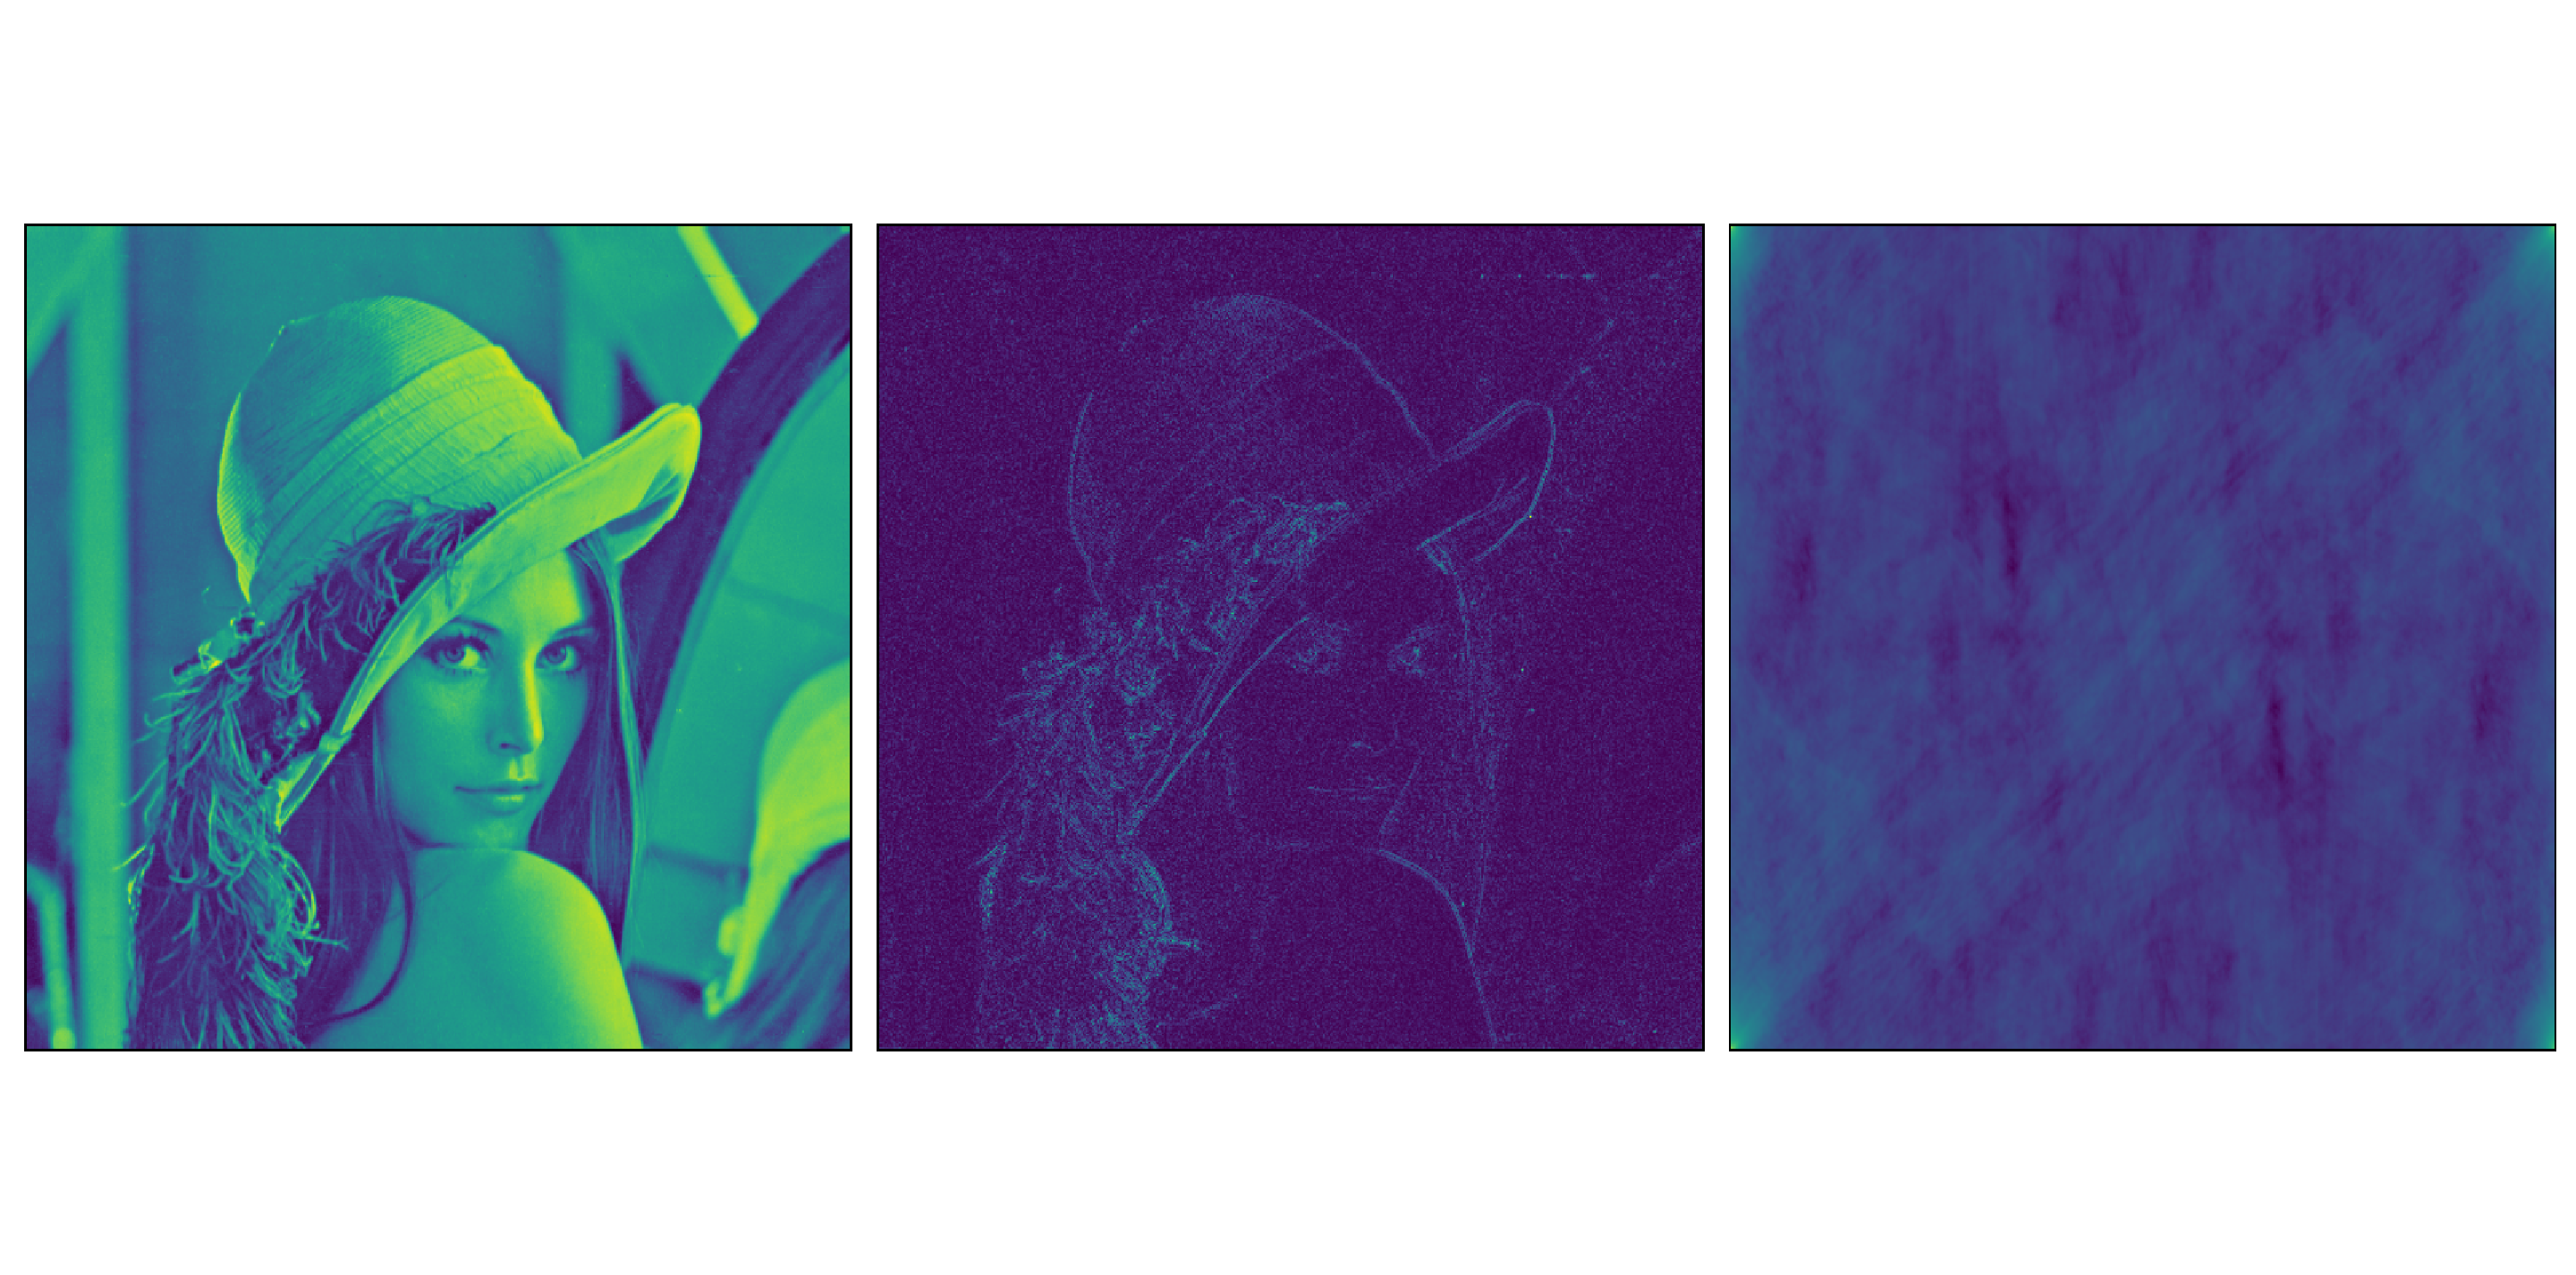
\includegraphics[width=.95\textwidth, trim=0 100 0 100, clip]{papers/kugel/figures/python/phase_vs_abs.pdf}
  \caption {
    From left to right: Greyscale image of Lena Forsén, reconstructed image
    using spectrum phase only, reconstructed image using spectrum magnitude
    only. Note that all image are actually greyscale but they are shown using
    a blue to yellow color map, because it has a better contrast that makes it
    easier to small details.
    \label{kugel:fig:2d-fourier-phasevsmagn}
  }
\end{figure}

With regard to images, on the other hand, the human eye does not work in this
way. The visual information that it extracts is not mathematically 'coded' in 
the same way as the eye does. We will then not have a situation in which the 
amplitude contains much more information than the phase does. In this case
we even have the opposite phenomena:
the phase of the Fourier transform of an image contains much more information
than the magnitude. This is very inconvenient for humans, as we usually start
by studying Fourier for signals in one dimension. So when one starts working
with images, the mindset must be changed, since most of the visual information
of an image is contained in the entity we know least about, the
phase-spectrum. In figure \ref{kugel:fig:2d-fourier-phasevsmagn}, your eyes
can judge for themselves this interesting peculiarity.

\subsection{Laplacian Operator}
\label{kugel:sec:preliminaries:laplacian}

We will now have another quick disgression in the realm of multivariate
calculus to refresh the Laplacian operator, which has already come up many
times throughout the book. In $\mathbb{R}^3$ using cartesian coordinates
coordinates the Laplacian operator is
\begin{equation*}
  \nabla^2 = \frac{\partial}{\partial x}
    + \frac{\partial}{\partial y}
    + \frac{\partial}{\partial z}
    = \sum_i \frac{\partial}{\partial x_i}
    = \nabla \cdot \nabla,
\end{equation*}
where in the last step we remined that the Laplacian is also the divergence of
the gradient with the suggestive (ab)use of notation for the dot product. With
quite a lot of effort it is possible to show that in spherical coordinates
(shown a few pages later in figure \ref{kugel:fig:spherical-coordinates}) the
Laplacian becomes\footnote{This is not the only way to write the Laplacian in
spherical coordinates, see \ref{buch:pde:section:kugel} for a discussion.}
\begin{equation*}
    \nabla^2 =
      \frac{1}{r^2} \frac{\partial}{\partial r} \left(
        r^2 \frac{\partial}{\partial r}
      \right)
      + \frac{1}{r^2} \left[
          \frac{1}{\sin\vartheta} \frac{\partial}{\partial \vartheta} \left(
            \sin\vartheta \frac{\partial}{\partial\vartheta}
          \right)
        + \frac{1}{\sin^2 \vartheta} \frac{\partial^2}{\partial\varphi^2}
      \right].
\end{equation*}
As we will see later, being a second derivative the Laplacian is a measure of
curvature.

\subsection{Eigenvalue Problems}

The final topic for this section are eigenvalue problems. In a vector space
$V$ over $\mathbb{K}$, the \emph{eigenvalue problem} for an
operator\footnote{To avoid confusion we should mention that the symbol
$\square$ is used for a generic operator and \emph{not} the d'Alembert
operator presented in section
\ref{buch:pde:section:gleichungen-und-randbedingungen}. Though, of course,
there are (very interesting) eigenvalue problems for the d'Alembert operator
such as the Klein–Gordon equation, which the reader is encouraged to learn
about.} $\square$ is the equation
\begin{equation*}
  \square v = \lambda v
\end{equation*}
where we need so solve for both the \emph{eigenvalues} $\lambda \in
\mathbb{K}$ and the \emph{eigenvectors} $v \in V$. In a finite vector space
(classic example), such as $\mathbb{R}^n$ an operator could be a square
$n\times n$ matrix $A$, and the problem is usually solved by first equating
characteristinc polynomial $\det(A - \lambda I)$ to zero to find the
$\lambda$'s, and then solving for the eigenvectors $v$. If $\square$ is a
derivative, then we end up in the theory of (ordinary) differential equations,
and if $\square$ is a partial derivative, then we can use methods such as the
separation method discussed in section \ref{buch:pde:section:separation}.

% Whichever the case, the eigenvalue problem should be understood as a search
% for what \emph{does not change} (up to a scalar factor) when 
